
\section{Methods}

\subsection{The Modular Behaviour Box}

At the outset it was decided that the scale of the modular architecture would probably have to match a given animal model, given the vastly different size scales between rodents, cats and primates. Our animal model of choice is the rodent \emph{rattus norvegicus}, and all of our proposed design choices target its size scale. Small adjustments could, however, be reasonably made up to a point for other mammals of similar stature, such as mice.

The main component and interface of the modular box is the individual $1\times 1$ module (Figure \ref{fig:modules}A). This module defines a standardized footprint ($\SI{12}{\centi\meter}\times \SI{12}{\centi\meter}$), against which all other modules are measured. Every newly fabricated module is built to specification to match a multiple of this standardized footprint (e.g. it is possible to have $2\times 1$, $2\times 2$, $4\times 1$ or any other multiple combination of the standard size). Inside the module footprint the module designer places a single logical component of a behaviour box and ensures that it can operate in isolation. Figure \ref{fig:modules} shows some examples of reusable modules developed throughout the project.

\begin{figure}
\centering
\includestandalone[scale=0.90]{chapters/figuresChTools/modules}
\caption{Some examples of standardized behaviour modules. (\textbf{A}) Detail of a $1\times 1$ module mounted in support frame. Fixation is achieved by driving a screw through post-insertion nuts placed in the structural framing (see text). (\textbf{B}) Example reward port module which can be floor- or wall-mounted. All relevant electronics and water distribution circuits are assembled on the back of the module (not shown). (\textbf{C}) Wall-mounted reconfigurable obstacle course stepper module. Stepper motors mounted on the back of the module allow for dynamic reconfiguration of the orientation of each step. (\textbf{D}) Floor-mounted obstacle course step pair. Multiple of these modules can be tiled together to assemble obstacle courses of arbitrary length.}
\label{fig:modules}
\end{figure}

\begin{figure}
\centering
\includestandalone[scale=1.00]{chapters/figuresChTools/box}
\caption{Example of a linear shuttling box assembled from a $\SI{1}{\meter}\times \SI{1}{\meter}$ modular structure using reward port and obstacle course step modules.}
\label{fig:box}
\end{figure}

\begin{figure}
\centering
\includestandalone[scale=0.90]{chapters/figuresChTools/box3d}
\caption{Side view of the linear shuttling box.}
\label{fig:box3d}
\end{figure}

\begin{figure}
\centering
\includestandalone[scale=1.00]{chapters/figuresChTools/verticalBox}
\caption{Example of vertical assembly. (\textbf{A}) Detail of a $1\times 1$ wall-mounted platform module. (\textbf{B}) Example of a vertical maze configuration.}
\label{fig:verticalBox}
\end{figure}

One of the principal requirements for assembling a box is fastening all its components together. By having a standard footprint, it is possible to design a set of regularly spaced mounting points that allows the experimentalist to quickly generate an entirely new configuration by simply swapping modular components inside the box (Figure \ref{fig:box}, \ref{fig:box3d}). For this work, we took advantage of an existing aluminium structural framing system (Bosch Rexroth, DE) to build the common mounting points (Figure \ref{fig:modules}A). Modules are fastened against post-insertion nuts which are able to slide across the whole length of the aluminium rail. Each of the modules is fastened by four screws, one in each corner. In order to ensure modules can be tightly and securely fixed one next to the other, we used a system of regularly spaced double rails (Figure \ref{fig:box}). This gives the frame the flexibility to easily reposition and rearrange individual modules tiling the entire footprint of any arbitrarily large box.

If the support frame is laid out vertically, it is possible to create modular walls of arbitrary dimensions. Some of the modules can be mounted equally well on a vertical or horizontal configuration, such as reward ports (Figure \ref{fig:modules}B). The three-dimensionality of the design has even been exploited to create vertical mazes (Figure \ref{fig:verticalBox}) to great success.

Throughout the project we made the base of every module from \SI{5}{\milli\meter} acrylic pieces. While not an absolute requirement for the design, this choice of plastic material has the advantage that a laser cutter can be used to very quickly produce a large collection of custom-built modules. In addition, patterns can be engraved or cut on the base to provide additional mounting points for hardware embedded in the module. The use of such rapid prototyping fabrication tools alongside with off the shelf available electronic sensors and actuators meant we were able to completely redesign the entire behaviour box, sometimes in a matter of days.

\subsection{The Bonsai Framework}

All the results concerning the Bonsai framework have been published as:
\fullcite{Lopes2015a}
\bigskip

Modern scientific experiments crucially depend on the control and monitoring of many parallel streams of data. Multiple measurement devices, from video cameras, microphones, and pressure sensors to neural electrodes, must simultaneously send their data in real-time to a recording system. General purpose digital computers have gradually replaced many of the specialized analog and digital technologies used for this kind of data acquisition and experiment control, largely due to the flexibility of programming and the exponential growth in computing power. However, the serial nature of programming instructions and shared memory makes it a challenge, even for experienced programmers, to develop software that can elegantly deal with the asynchronous, parallel nature of scientific data.

Another challenge arises from the need for software integration. Each hardware vendor provides their own set of drivers and programming interfaces for configuring and acquiring data from their devices. In addition, the growth of the open-source movement has greatly increased the number of freely available technologies for different data processing domains. Integration of these diverse software and hardware components remains a major challenge for researchers.

These difficulties lead to increased development times when setting up an experiment. Moreover, it requires experimenters to pursue specialized training outside their domain of research. This limits the ability to rapidly prototype and try out new designs and can quickly become the factor limiting the kinds of questions that are amenable to scientific investigation.

Here we describe Bonsai, an open-source visual programming framework for processing data streams. The main goal of Bonsai is to simplify and accelerate the development of software for acquiring and processing the many heterogeneous data sources commonly used in (neuro) scientific research. We aim to facilitate the fast implementation of state-of-the-art experimental designs and to encourage the exploration of new paradigms. The framework has already been successfully used for many applications. In the following we will specifically highlight Bonsai's utility in neuroscience for monitoring and controlling a diverse range of behaviour and physiology experiments.

\subsubsection{Architecture}

Scientific data, like the world we live in, is inherently parallel. To monitor this complexity, modern experimenters are often forced to use multiple electronic instruments simultaneously, each with their own independent sampling rates. As data arrives at the acquisition computer, there are two main approaches to log and process these asynchronous data streams. The first approach is to use a polling strategy: a single sequential process in the computer runs a processing loop that goes through each device in sequence and gathers the available data. In this case, data from only one device is being collected and manipulated at any point in time. The second approach is to use an event-driven (reactive) architecture: processes are setup in parallel to collect data from all the devices simultaneously. Whenever new data is available, notifications are sent to the appropriate software routines that collect and process the data as soon as possible. When only a single processor is available, the difference between these two strategies is negligible: only one instruction at a time can be executed by the computer. However, with modern multi-processor cores and dedicated data transfer circuits, the performance difference between the two approaches will significantly influence the throughput of a data acquisition and processing system. Unfortunately, software tools to support and facilitate the “reactive” approach to data stream processing are only just now starting to be adopted and most software systems are still built from the sequential composition of simple program routines. Many of the assumptions of the sequential processing scenario do not scale to handle parallel execution, especially when shared memory and resources are involved.

In recent years, a number of advances in programming languages and software frameworks have tried to make it easier to create complex software applications by composition of asynchronous computing elements \cite{Bainomugisha2013}. Bonsai builds upon these new efforts and aims to extend these developments to the rapid-prototyping domain by introducing a visual programming language for composing and processing asynchronous data streams. Bonsai was developed on top of the Reactive Extensions for the.NET framework (Rx) \cite{MicrosoftOpenTechnologies2014}. Rx provides many built-in operators that transparently deal with the concurrency challenges that inevitably surface when multiple data streams need to be processed and integrated together in a single program. It has become an increasingly popular framework to develop reactive interfaces for next generation mobile and desktop computing platforms, where it is used to handle the growing number of sensors and network communications required by business logic and consumer applications.

Bonsai (via Rx) represents asynchronous data streams using the notion of an observable sequence. An observable sequence represents a data stream where elements follow one after the other. An example would be a sequence of frames being captured by a camera, or a sequence of key presses logged by the keyboard. The name observable simply specifies that the way we access elements in the data stream is by listening to (i.e., observing) the data as it arrives, in contrast with the static database model, in which the desired data is enumerated.

In Bonsai, observable sequences are created and manipulated graphically using a dataflow \cite{Mosconi2000, Johnston2004} representation (Figures \ref{fig:bonsaiInterface}, \ref{fig:bonsaiExamples}A, Supplementary Video 1). Each node in the dataflow represents an observable sequence. Nodes can be classified as either observable sources of data or combinators (Table \ref{tab:bonsaiCategories}). Sources deliver access to raw data streams, such as images from a video camera or signal waveforms from a microphone or electrophysiology amplifier. Combinators represent any observable operator that handles one or more of these sequences. This category can be further specialized into transforms, sinks and other operator types depending on how they manipulate their inputs (Table \ref{tab:bonsaiCategories}). Transforms modify the incoming data elements of a single input sequence. An example would be taking a sequence of numbers and generating another sequence of numbers containing the original elements multiplied by two. Sinks, on the other hand, simply introduce processing side-effects without modifying the original sequence at all. One example would be printing each number in the sequence to a text file. The act of printing in itself changes nothing about the sequence, which continues to output every number, but the side-effect will generate some useful action. Combinators that change, filter or merge the flow of data streams are neither transforms nor sinks, and they are simply referred to by the more general term combinator. The Sample combinator illustrated in Figure \ref{fig:bonsaiExamples}A takes two data sequences and produces a new sequence where elements are sampled from the first sequence whenever the second sequence produces a new value. In this example, we use Sample to extract and save single images from a video stream whenever a key is pressed.

\begin{figure}
\begin{center}
\scalebox{0.7}{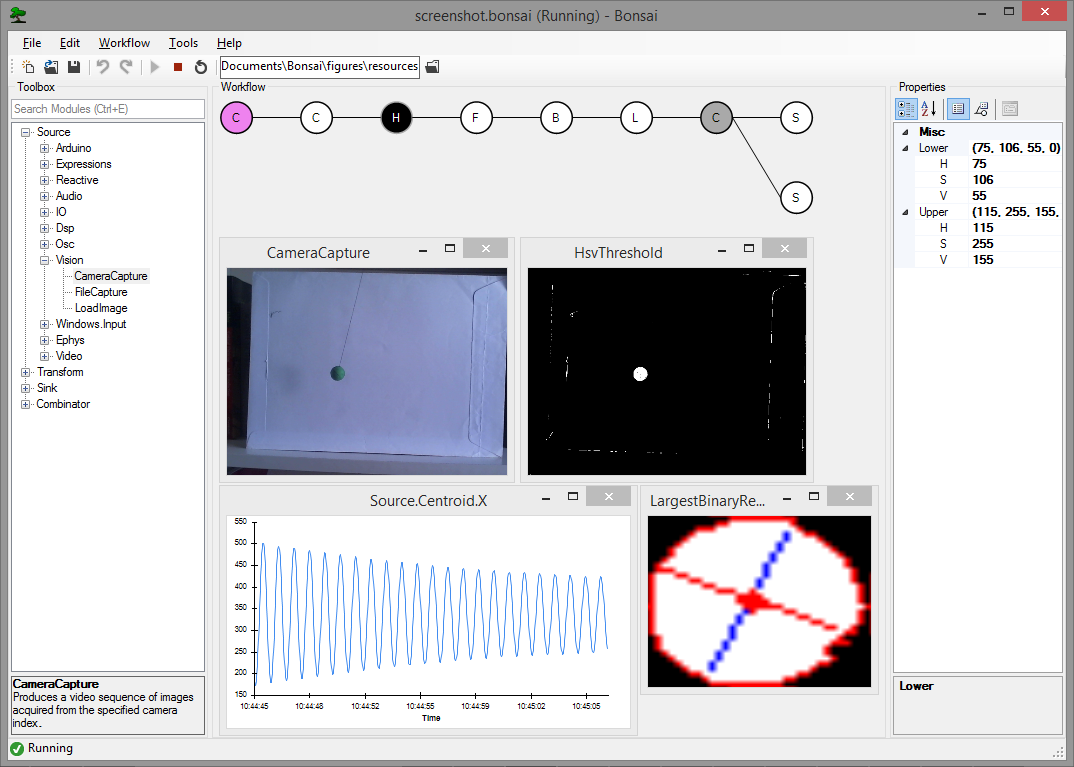
\includegraphics[width=\linewidth]{chapters/figuresChTools/bonsaiInterface.png}}
\end{center}
\vspace{-5mm}
\caption{Screenshot of the Bonsai user interface running a video processing pipeline. An example dataflow for color segmentation and tracking of a moving pendulum is shown. Data sources are colored in violet; transform operators in white; sinks in dark gray. The currently selected node (HsvThreshold) is colored in black and its configuration parameters are displayed in the properties panel on the right. Overlaid windows and graphs represent Bonsai data visualizers for the output of individual nodes.}
\label{fig:bonsaiInterface}
\end{figure}

\begin{figure}
\begin{center}
\scalebox{0.5}{\includesvg{chapters/figuresChTools/bonsaiExamples}}
\end{center}
\vspace{-5mm}
\caption{Examples of dataflow processing pipelines using Bonsai. \textbf{(A)} Taking grayscale snapshots from a camera whenever a key is pressed. Top: graphical representation of the Bonsai dataflow for camera and keyboard processing. Data sources are colored in violet; transform operators in white; combinators in light blue; sinks in dark gray. Bottom: marble diagram showing an example execution of the dataflow. Colored tokens represent frames arriving from the camera. Black circles represent key press events from the keyboard. Asterisks indicate saving of images to permanent storage. \textbf{(B)} Dynamic modulation of an image processing threshold using the mouse. The x-coordinate of mouse movements is used to directly set the externalized ThresholdValue property (orange). The updated threshold value will be used to process any new incoming images. \textbf{(C)} Grouping a set of complex transformations into a single node. In the nested dataflow, the source represents incoming connections to the group and the sink represents the group output.}
\label{fig:bonsaiExamples}
\end{figure}

\begin{table}
\begin{center}
\scalebox{0.7}{\includesvg{chapters/figuresChTools/bonsaiCategories}}
\end{center}
\vspace{-5mm}
\caption{List of Bonsai node categories. The color of each Bonsai node serves as a visual aid to identify their role in dataflow processing pipelines. Most of these categories are actually specializations of the very general combinator and are meant to visually depict their specific data processing semantics.}
\label{tab:bonsaiCategories}
\end{table}

A common requirement when designing and manipulating dataflows is the ability to visualize the state of the data at different stages of processing. We have therefore included a set of visualizers to assist debugging and inspection of data elements, including images and signal waveforms (Figure \ref{fig:bonsaiInterface}). These visualizers are automatically associated with the output data type of each node and can be launched at any time in parallel with the execution of the dataflow. Furthermore, it is often desirable to be able to manipulate processing parameters online for calibration purposes. Each node has a set of properties which parameterize the operation of that particular source or combinator (Figure \ref{fig:bonsaiInterface}). This allows, for example, changing the cutoff frequency of a signal processing filter, or setting the name of the output file in the case of data recording sinks. We have also included the possibility of externalizing node properties into the dataflow (Figure \ref{fig:bonsaiExamples}B). Externalizing a property means extracting one of the parameters into its own node in the dataflow, making it possible to connect the output of another node to the exposed property. This allows for the dynamic control of node parameters.

Finally, we have built into Bonsai the ability to group nodes hierarchically. In its simplest form, this feature can be used to encapsulate a set of operations into a single node which can be reused elsewhere (Figure \ref{fig:bonsaiExamples}C). This is similar to defining a function in a programming language and is one of the ways to create new reactive operators in Bonsai. Any named externalized properties placed inside an encapsulated dataflow will also show up as properties of the group node itself. This allows for the parameterization of nested dataflows and increases their reuse possibilities. In addition, encapsulated dataflows are used to specify more complicated, yet powerful, operators such as iteration constructs that allow for the compact description of complex data processing scenarios that can be cumbersome to specify in pure dataflow visual languages \cite{Mosconi2000} (see below).

Bonsai was designed to be a modular framework, which means it is possible to extend its functionality by installing additional packages containing sources and combinators developed for specific purposes. New packages can be written using C\# or any of the.NET programming languages. Python scripts [via IronPython \cite{IronPython2014}] can be embedded in the dataflow as transforms and sinks, allowing for rapid integration of custom code. All functionality included in Bonsai was designed using these modular principles, and we hope to encourage other researchers to contribute their own packages and thereby extend the framework to other application domains. At present, the available packages include computer vision and signal processing modules based on the OpenCV library \cite{Itseez2014}. Drivers for several cameras and interfaces to other imaging and signal acquisition hardware were integrated as Bonsai sources and sinks, including support for Arduino microcontrollers \cite{Banzi2014}, serial port devices and basic networking using the OSC protocol \cite{Wright2003}. Given the specific applications in the domain of neuroscience, we also integrated a number of neuroscience technology packages. The Ephys package, for example, builds on the Open Ephys initiative for the sharing of electrophysiology acquisition hardware \cite{Voigts2013} by providing support for the Rhythm open-source USB/FPGA interface (Intan Technologies, US). Therefore, the next generation tools for electrophysiology can already be used inside Bonsai, the acquired physiology data implicitly integrated with other available data streams and thus easily assembled into a powerful and flexible experimental neuroscience platform.

\subsubsection{Advanced Operators}

The most common application of Bonsai is the acquisition and processing of simple, independent data streams. However, for many modern experiments, basic acquisition and storage of data is often not sufficient. For example, it can be convenient to only record the data aligned on events of interest, such as the onset of specific stimuli. Furthermore, neuroscience experiments often progress through several stages, especially for behavioral assays, where controlled conditions vary systematically across different sessions or trials. In order to enforce these conditions, experiments need to keep track of which stage is active and use that information to update the state of control variables and sensory processing. These requirements often cannot be described by a simple linear pipeline of data, and require custom code to handle the complicated logic and bookkeeping of experimental states. Below we describe a set of advanced Bonsai operators that can be used to flexibly reconfigure data processing logic to cover a larger number of scenarios. These operators and their applications are all built on the single idea of slicing a data stream into sub-sequences, called windows, which are then processed independently and, potentially, in parallel (Figure \ref{fig:bonsaiAdvanced}).

\begin{figure}
\begin{center}
\scalebox{0.5}{\includesvg{chapters/figuresChTools/bonsaiAdvanced}}
\end{center}
\vspace{-5mm}
\caption{Using slicing and window processing combinators in Bonsai.}
\label{fig:bonsaiAdvanced}
\end{figure}

Bonsai provides different combinators that allow the creation of these sub-sequences from any observable data stream, using element count information, timing, or external triggers (Figures \ref{fig:bonsaiAdvanced}A–C). The specific set of operations to apply on each window is described by encapsulating a dataflow inside a SelectMany group, as detailed in the signal processing example of Figure \ref{fig:bonsaiAdvanced}D. The input source in this group represents each of the window sub-sequences, i.e., it is as if each of the windows is a new data source, containing only the elements that are a part of that window. These elements will be processed as soon as they are available by the encapsulated dataflow. Windows can have overlapping common elements, in which case their processing will happen concurrently. The processing outputs from each window are merged together to produce the final result. In the case of Figure \ref{fig:bonsaiAdvanced}D, past and future samples are grouped in windows to compute a running average of the signal through time, necessarily time-shifted by the number of future samples that are considered in the average.

The processing of the elements of each window happens independently, as if there was a new isolated dataflow running for each of the sequences. We can exploit this independence in order to dynamically turn dataflows on and off during an experiment. In the video splitting example of Figure \ref{fig:bonsaiAdvanced}E, we use an external trigger source to chop a continuous video stream into many small video sequences, aligned when the trigger fired. We then nest a VideoWriter sink into the SelectMany group. The VideoWriter sink is used to encode video frames into a continuous movie file. It starts by creating the video file upon arrival of the first frame, and then encoding every frame in the sequence as they arrive. When the data stream is completed, the file is closed. By nesting the VideoWriter inside the SelectMany group, what we have effectively done is to create a new video file for each of the created windows. Whenever a new trigger arrives, a new clip is created and saving proceeds, implicitly parallelized, for that video file.

More generally, we can use this idea to implement discrete transitions between different processing modes, and chain these states together to design complex control structures such as finite state machines (FSMs). FSMs are widely used to model environments and behavioral assays in systems and cognitive neuroscience. One example is illustrated in Figure \ref{fig:bonsaiAdvanced}F, where we depict the control scheme of a stimulus-response apparatus for a simple reaction time task. In this task, there are only two states: Ready and Go. In the Ready state, no stimulus is presented and a timer is armed. Whenever the timer fires, the task transitions into the Go state, and a stimulus is presented. The subject is instructed to press a key as fast as possible upon presentation of the stimulus. As soon as the key is pressed, the system goes back to the Ready state to start another trial. In a FSM, nodes represent states, e.g., stimulus availability or reward delivery, and edges represent transitions between states that are caused by events in the assay, e.g., a key press. In each state, a number of output variables and control parameters are set (e.g., turning on a light) which represent the behaviour of the machine in that state.

In the Bonsai dataflow model, dataflows encapsulated in a SelectMany group can be used to represent states in a FSM (Figure \ref{fig:bonsaiAdvanced}F, bottom). Specifically, a state is activated whenever it receives an input event, i.e., the dataflow nested inside the state will be turned on. The dynamics of the nested dataflow determine the dynamics of the state. In the Go state presented in Figure \ref{fig:bonsaiAdvanced}F, the activation event is used to trigger stimulus onset. In parallel, we start listening for the key press which will terminate the state. Conversely, for the Ready state we would trigger stimulus offset and arm the timer for presenting the next stimulus. An important difference between Bonsai dataflows and pure state machine models is that a dataflow is specified as a directed acyclic graph, i.e., the data stream cannot loop back on itself. However, by taking advantage of the Repeat combinator, we can restart a dataflow once it is completed, allowing us to reset the state machine for the next trial.

Many of the control tasks in experiments have this sequential trial-based structure, which has allowed us to rapidly prototype complex behaviour assays, such as closed-loop rodent decision making tasks, simply by leveraging the flexibility of the data stream slicing operators.

\subsubsection{Alternatives to Bonsai}

Although graphical user interfaces have played a crucial role in the widespread proliferation of computing technology throughout various scientific fields, the majority of these interfaces tend to be applied to relatively narrow domains, such as the operation of a specific instrument. Their goal is often to provide access to all the various configuration parameters of the hardware and to provide basic data acquisition functionality. There is often no opportunity to parameterize or condition the behaviour of the instrument beyond the possibilities presented by the interface, and interconnections with other devices are often limited to simple hardware triggers. The alternative, when available, is to access low-level application programming interfaces (APIs), and program the desired behaviour from scratch.

In the more flexible domains of data analysis, behaviour control and software simulations, the use of more versatile graphical interfaces has become increasingly prevalent. In these scenarios, it is not uncommon to encounter the development of domain-specific languages (DSLs), where graphical building blocks related to the domain of application can be combined together by the user to generate new behaviors, such as the sequence of steps in a psychophysics experiment or a state-machine diagram used to control stimuli and rewards in operant conditioning. While providing more flexibility to the end user, such DSLs are usually not conceived, at their core, to be applied to wildly different domains (e.g., an operant conditioning state machine is not expected to be able to filter continuous electrophysiology signals). In fact, most DSLs will not even allow the user to extend the set of built-in operations. In those that do, the developer may find a customization pit \cite{Cook2007}, where concepts and operations that are within the range of what the DSL can express are easy to develop, whereas tasks that are a little bit outside of the boundaries of the language quickly become impossible or too cumbersome to implement.

As the level of flexibility of a graphical user interface increases, we start to approach the space occupied by general purpose visual programming languages (GPVPL). These are languages that are designed from the outset to be capable of solving problems across a wide variety of domains using a general set of operations. Ideally, the core building blocks of the language will themselves be domain-independent, so that the user can easily apply the same set of operations to the widest possible class of inputs. In order to better illustrate the feel and expressive power of GPVPLs, and to clarify where Bonsai itself is positioned, we will give two examples of popular languages that have succeeded in this niche: LabVIEW \cite{Instruments2014} and Simulink \cite{MathWorks2014}.

LabVIEW is one of the best examples of a GPVPL applied to the design and control of experiments \cite{Elliott2007}. In LabVIEW, users create virtual instruments (VIs) which are composed of a graphical front-panel containing an assortment of buttons, dials, charts and other objects; as well as a back-panel where a flowchart-like block diagram can be used to specify the behaviour of the VI. In this back-panel, nodes and terminal elements can represent hardware components, numerical operations or front-panel objects, which are connected together using virtual wires that specify the flow of data between them. The popularity of LabVIEW grew initially from its support for state-of-the-art data acquisition cards and hardware as well as its data visualization capabilities. The modularity of its architecture also allowed users to quickly develop and implement new nodes within the language itself by using VIs themselves as nodes.

Although the LabVIEW back-panel is a dataflow visual programming language, its execution model tends to follow a polling, rather than event-driven, strategy for dealing with multiple data streams. In order to properly scale this model to the increasing number of available processor cores, LabVIEW has implemented sophisticated code analysis tools that attempt to identify parallelizable portions of block diagrams automatically (Elliott et al., 2007). Once these sections are identified, LabVIEW will automatically generate parallel processes depending on the number of available cores and will manage the bottlenecks in the code accordingly. Although this mitigates the limitations of the sequential polling programming model, it is important to realize that the goal of such automatic parallelization is still to provide the user with a logically synchronized programming model.

Simulink is a popular dataflow visual programming language for modeling, simulating and analyzing multi-domain dynamic systems. It has become extremely popular for modeling response characteristics of control systems, allowing not only for the rapid prototyping of algorithms, but also the automatic generation of microcontroller code for embedded systems. Again, the success of the language stemmed primarily from the flexibility and ease of use of the block diagrams, as well as the number of prebuilt operations and data visualization tools which quickly took care of many crucial but tedious aspects of control systems modeling.

Like LabVIEW, the execution model for Simulink generated code is still based on polling strategies, where ready to execute dataflow nodes are updated in turn as inputs become available. Again, strategies to scale the output of Simulink to multiple cores have been proposed based on analyzing and segmenting the model into parallelizable sections which can be converted into equivalent parallel execution code for microcontrollers \cite{Kumura2012}.

Similar to LabVIEW and Simulink, Bonsai was designed as a general purpose modular language. The core architecture of Bonsai is domain-independent and provides a general framework to compose asynchronous data streams. A general set of composition operators, or combinators, provides support for iteration, segmentation and merging of parallel data streams, as well as other common manipulations on observable sequences. Both the sources of data and available processing operations can be extended within the language itself using nesting of dataflows. Data visualizers and a growing library of data stream acquisition, processing and logging modules are provided to allow rapid prototyping of a large number of different applications.

However, in contrast to LabVIEW or Simulink, Bonsai adopts a very different strategy to implement dataflow execution. Rather than trying to derive a global sequential execution order of dataflow nodes based on the number of active inputs, Bonsai nodes simply react to incoming inputs immediately, without the need to wait for all of them to be active. When multiple observable sequences are present, this allows for a choice of different concurrency composition strategies. Nevertheless, as the result of the composition is an observable sequence itself, such concurrency management can remain functionally isolated from the combinator that is handling the composition. From the point of view of downstream operators, they are simply receiving an observable sequence. There is a tradeoff, of course, that more responsibility for managing the flow of data is passed to the end user, but it also allows for a finer grained control of concurrency that is critical to the specification of parallel applications.

One important caveat of developing asynchronous systems is that debugging can be more difficult in situations where the precise timing and ordering of events is required to reproduce an offending behaviour. In synchronized and sequential execution environments, one can easily go step by step through the precise cascade of transformations that resulted in a problem. In contrast, when multiple processes are executing concurrently, it can be harder to analyze the program flow in a similarly reproducible, deterministic manner. However, it should be noted that this issue is not unique to reactive environments with real asynchronous devices. A sequential polling strategy will be equally deficient in reproducing a particular execution sequence when data from parallel input devices is being accessed.

Another important caveat is that Bonsai currently runs exclusively in Windows operating systems. However, Microsoft has recently open-sourced the execution engine of the.NET framework and will pursue implementations for all the major operating systems (Linux/Mac). This raises the interesting possibility of eventually extending the Bonsai user base into these important platforms.